\documentclass[a4paper]{scrartcl}
\usepackage[utf8]{inputenc}
\usepackage{xcolor}
\usepackage{graphicx}
\graphicspath{{./figures/}}

\title{Assignment 1}
% \textcolor{gray}{Critique and re-design of an existing graphic}
\author{Alina Mokrova\\
				id
				\and
				Levente	Slajchó\\
				id
				\and
				Maximilian Walterskirchen\\
				id
				\and
				Leminh Nguyen\\
				11945068}
\date{\today}

\begin{document}

\maketitle

\section{Analysis and criticism}


\subsection{Analysis of this graphic}

The infographic \textit{Nutritional Values} by Dan Mariglio in
Figure~\ref{assignmentGraphic} pictures the nutritional comparison between
processed and natural/wholesome food. The author visualizes three different
infographics for the different food categories; the first graph compares the
cost per calorie, another one contrasts the calories per \textit{100g} and the
last shows how much sugar is contained in \textit{100g}. The author gives the
example that wholesome food is more expensive since the ratio of value to
calorie for an apple is higher compared to a bag of potato chips. Mariglio based
his visualizations on the layout of common supermarkets and suggests the reader
sticking to the periphery of the supermarket to find the natural food.
Processed food containing the most calories by weight is located at the centre
of the grocery store.

\subsection{Criticism of the visual design}

%      In a first step you should argue why the given presentation is not
%       appropriate to represent the data in an efficient way. Please argue about
%       the deficiencies of the graphic with respect to the design principles we
%       covered in the lecture (Data-Ink-Ratio, Visual Clutter, ...).  Hand in a
%       short text about your argumentation.

% \textcolor{gray}{To deal with a given static graphic, to identify deficiencies
% of the visual representation, and to find a more suitable way to present the
% data at hand.}

In this section, the three sub-infographics will be criticised according to the
information design principles from the lecture notes.

% Some notes:
% \begin{itemize}
%      The author uses the \textit{Bottom up} approach which is data driven
%      The graphics is a conventional representation an used the controlled visualization paradigm (reason: data driven)
%      Which requires the attentive perception of the reader/viewer
%      Attentive approach is slow to perceive and easy to forget information
%      Based on visual processing paradigm and requires the following from the viewer:
%     \begin{itemize}
%          Parallel processing to extract low level properties of the visual scene
%          Pattern perception
%     \end{itemize}
%      Deficiency for viewers with color blindness, see produce aisle/section which is represented in red and green
%      Graphic in 3 dimensions which makes it way more complex than it is
%      The food graphical components obscure the actual information and data $\rightarrow$ hard to perceive actual infographic
%      Preattentive processing:
%     \begin{itemize}
%          No immediate understanding
%          No preattentive attributes except for food labels, but many are obscured by other components
%          Hard for immediate perception
%     \end{itemize}
%      The perspective suggests the entry of the store in the graphic is on the right side, and that the higher numbers of the table are closer in perspective $\rightarrow$ based on the western left to right reading perspective it should be the other way around
%      The differences between the three tables are difficult to compare due to too much information and bright color
%      Data-Users-Tasks triangle:
%     \begin{itemize}
%          Expressiveness - Are the visual elements expressive enough? $\rightarrow$ Even too much
%          Effectiveness - Is the information displayed effectively? $\rightarrow$ Not at all
%          Appropriateness - Is the visualization appropriate? $\rightarrow$ Yes, it's perfect for the subject
%     \end{itemize}
% \end{itemize}

\section{Assessment of redesign}

%      In a third step you should argue why you chose to represent the data
%       that way. What did you change? Why is this representation better suited
%       than the original one? Hand in a short text about your argumentation.

% link to appendix of new design

\bibliographystyle{ieeetr}
\bibliography{ivassignment}

\newpage
\clearpage
\section{Appendix}

\begin{figure}[h]
  \centering
	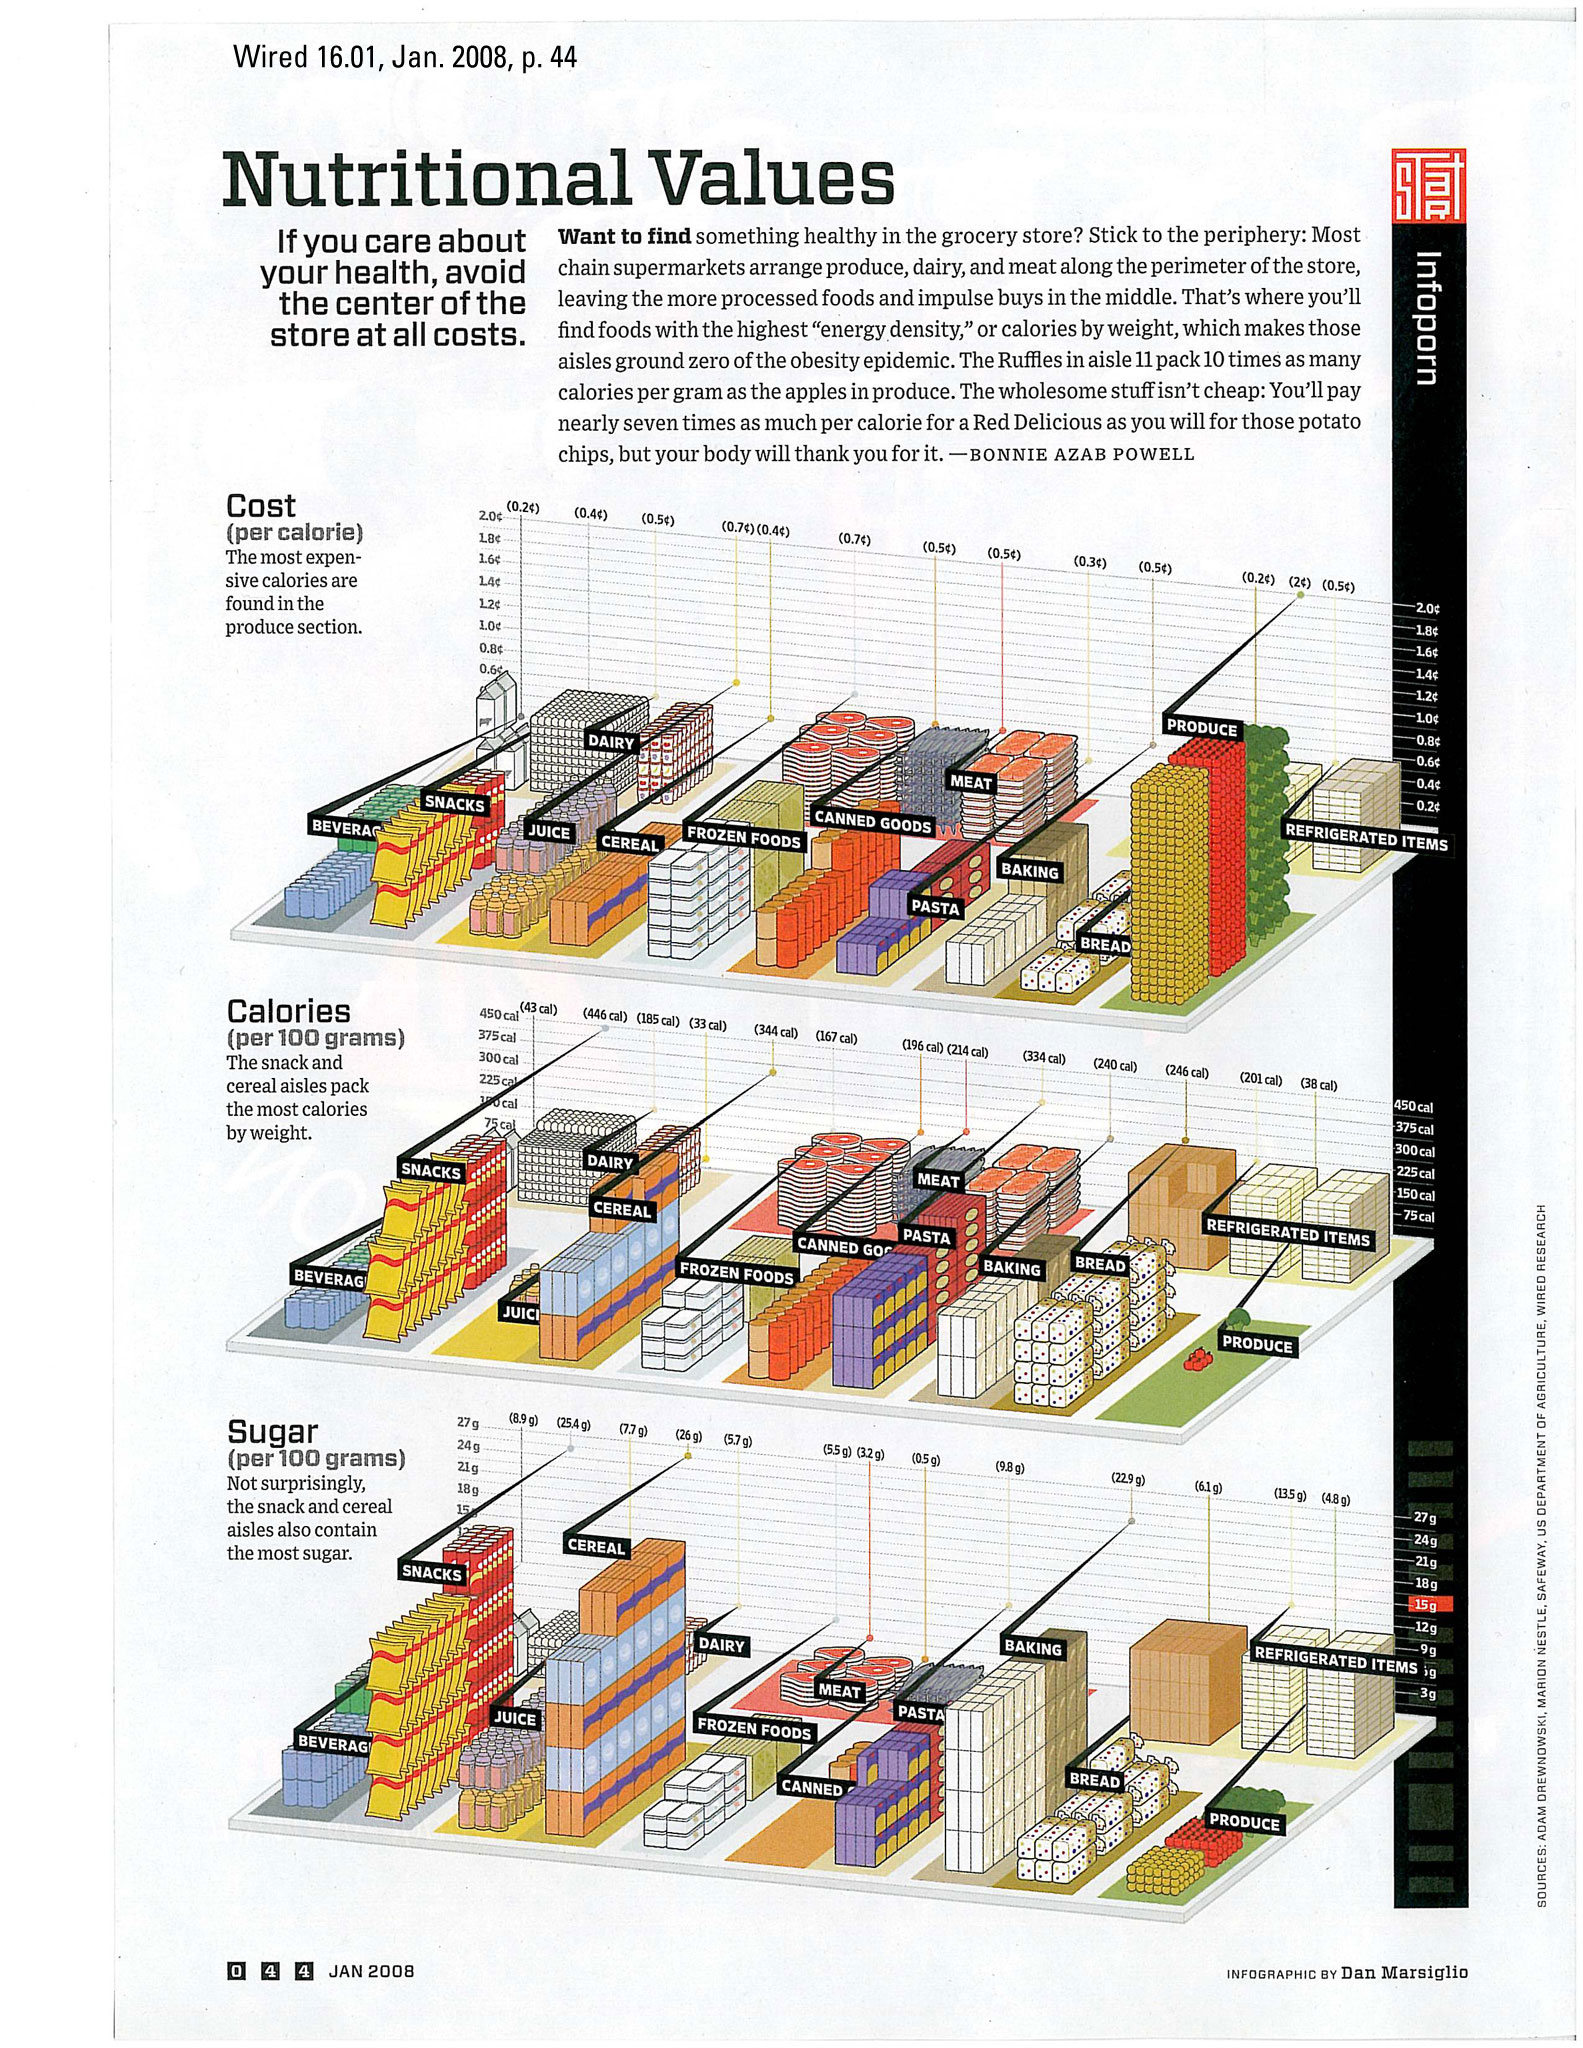
\includegraphics[scale=0.20]{assignmentGraphic.jpg}
  \caption{Given graphic to criticize.}
	\label{fig:assignmentGraphic}
\end{figure}

\end{document}
